\documentclass[10pt,a4paper]{article}
\usepackage[margin=2.2cm]{geometry}
\usepackage[T1]{fontenc}
\usepackage{graphicx}
\usepackage{booktabs}
\usepackage{amsmath}
\usepackage[hidelinks]{hyperref}
\usepackage{xcolor}
\usepackage[numbers,sort&compress]{natbib}

\title{Leakage and Label Noise Inflate UAV Flight-Log Diagnosis:\\
A Verifiable Real-Failure Benchmark for ArduPilot}
\author{AUTHOR NAME\\ AFFILIATION\\ \texttt{EMAIL}}
\date{Draft --- \today}

\begin{document}
\maketitle

\begin{abstract}
Automated root-cause diagnosis of small-UAV crashes from onboard flight logs
is often reported with high accuracy. We show, on real ArduPilot failure logs,
that such figures are produced by evaluation practice rather than diagnostic
skill. First, we audit forum-mined crash labels against the discussion
threads they came from. Of 55 logs previously treated as labelled, only 24
have a cause stated in their thread, and those agree only weakly with the
original labels (Cohen's $\kappa = 0.39$). The audit also found a simulated
flight listed as a real crash, labels swapped between files, and a label
derived from post-impact sensor noise. Second, we release a benchmark of
34 real logs from 32 incidents. Every label cites a verbatim forum post and
can be re-verified automatically. Third, in a pre-registered evaluation, the
same classifiers score 0.78--0.97 macro-F1 when windows of one flight are
split at random, and 0.06--0.07 when incidents are kept intact, against a
random-guess baseline of 0.08. No evaluated method, including a hybrid
rule/ML engine with temporal root-cause arbitration, exceeds chance. Error
analysis shows the rule engine labels the downstream symptoms of a failed
motor (a power drop, compensating outputs) instead of the failure itself.
We release code, labels and a one-command reproduction.
\end{abstract}

\section{Introduction}
Operators of ArduPilot-based vehicles \citep{ardupilot} usually diagnose
crashes by posting a DataFlash log to the community forum
\citep{ardupilotforum}, where experienced users read the telemetry by hand.
Automating this step is attractive, and several open tools claim to do it.
Measuring whether they work is harder than it looks:
\begin{itemize}
\item Real crash logs are scarce.
\item Labels are usually mined from forum text.
\item A single flight yields many correlated windows.
\end{itemize}
These are the classic conditions for evaluation leakage
\citep{kapoor2023leakage} and benchmark label noise
\citep{northcutt2021labelerrors}.

This paper is a self-audit of one such tool, an open-source hybrid
rule/ML ArduPilot log diagnoser. Its published accuracy fell from
\emph{1.0} to \emph{chance} as evaluation errors were removed. We make four
contributions:
\begin{enumerate}
\item \textbf{A label audit} of forum-mined crash labels against their source
      threads (Section~\ref{sec:audit}).
\item \textbf{A verifiable benchmark:} each label carries a permalink and a
      verbatim quote, checked automatically (Section~\ref{sec:data}).
\item \textbf{A pre-registered leakage study} showing a ten-fold inflation
      from window-level splitting (Section~\ref{sec:leak}).
\item \textbf{An error analysis} explaining why rule-based diagnosis names
      symptoms rather than causes (Section~\ref{sec:errors}).
\end{enumerate}

\section{Related work}
UAV fault datasets such as ALFA \citep{keipour2019alfa} and RflyMAD
\citep{le2023rflymad} provide fault-injection or simulated flights with known
fault times. BASiC \citep{basic2024} provides simulated ArduCopter failures.
Such data are valuable, but a near-perfect score on scripted simulator faults
does not transfer to organic field crashes. The tool audited here reported
exactly such a score. Leakage through non-independent splits is a documented
cause of irreproducible ML results across science \citep{kapoor2023leakage}.
Label errors in test sets can reorder method rankings
\citep{northcutt2021labelerrors}. We document both effects in a new domain.

\section{The audited system and its reporting history}
The tool parses DataFlash logs and extracts 111 features in 5\,s windows
with 50\% overlap. It combines a threshold rule engine, a tree classifier and
an anomaly detector. A temporal arbitration step (CITA) chooses as root cause
the diagnosis whose anomaly began earliest. Table~\ref{tab:history} lists the
headline figures the project published over time, and why each was
withdrawn. All corrections are public in the repository.

\begin{table}[h]\centering\small
\caption{Reported headline accuracy of the audited tool over time.}
\label{tab:history}
\begin{tabular}{p{3.4cm}p{1.3cm}p{9.6cm}}
\toprule
Claim & Macro-F1 & Why it does not hold\\\midrule
Simulated BASiC set & 1.00 & Scripted simulator faults, not real crashes\\
``Release'' benchmark & 0.81 & All 6 evaluated logs were in the training set\\
Filename-grouped split & 0.67 & Windows of one incident crossed the split\\
URL-grouped split & 0.56 & Contradictory labels, mostly created by rule-engine relabelling\\
``Honest'' candidate & 0.50 & Pool included simulated flights; artefacts never committed\\
This work (v3) & 0.06--0.07 & Real logs, incident-grouped, thread-verified labels\\
\bottomrule
\end{tabular}
\end{table}

\section{Label audit}\label{sec:audit}
The tool's real-log labels came from forum threads. Some came from staff
diagnoses, many from the search query used to find a thread, and three had
been silently overwritten by the tool's own rule engine. We fetched every
cited thread and re-labelled each log from the thread alone.

\textbf{Protocol.} A label requires a post, by someone other than the
original poster, that names a cause. Alternatively, the original poster may
confirm a cause found after investigation. Competing causes without
resolution give \emph{undiagnosed}. Each label records:
\begin{itemize}
\item the post permalink, author and forum role;
\item a verbatim quote;
\item a certainty: \emph{explicit} or \emph{tentative} (hedged wording).
\end{itemize}
Label definitions follow the tool's taxonomy. In particular, a sudden
single-motor, ESC or propeller loss is \texttt{mechanical\_failure}, not
\texttt{motor\_imbalance}.

\textbf{Annotator disclosure.} All labels were assigned by a large language
model reading the threads. They have \emph{not yet} been reviewed by a
human; a 10-item human spot-check is prepared. A script re-verifies every
quote against the thread text: 83 of 83 quotes matched the cached threads,
and randomly re-fetched posts matched live.

\begin{figure}[t]\centering
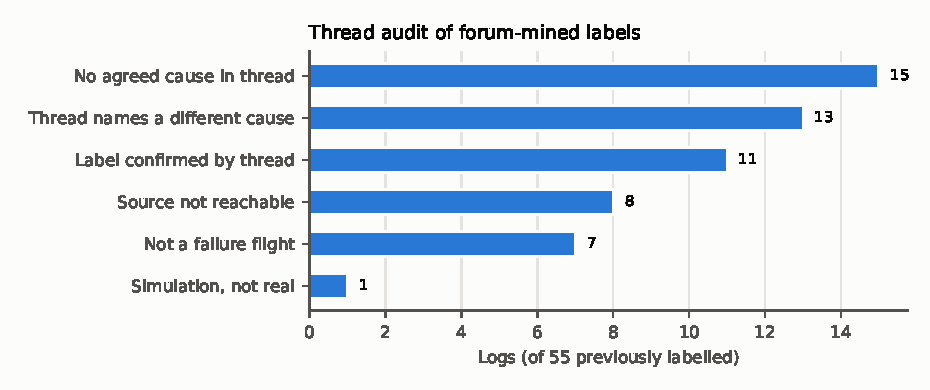
\includegraphics[width=0.8\linewidth]{figures/label_audit.pdf}
\caption{Outcome of re-labelling 55 previously labelled real logs from their
source threads.}\label{fig:audit}
\end{figure}

\textbf{Findings} (Fig.~\ref{fig:audit}):
\begin{itemize}
\item Of 55 logs, 24 have a cause stated in their thread: 11 confirm the old
      label and 13 change it (Cohen's $\kappa=0.39$ \citep{cohen1960kappa}).
\item 15 threads never agree on a cause, 7 logs are not failure flights,
      1 is a Gazebo simulation, and 8 sources were unreachable.
\item The most common correction is \texttt{motor\_imbalance} to
      \texttt{mechanical\_failure}.
\item In one thread, labels were swapped between the crash log and an
      uneventful post-crash flight.
\item In another, a GPS label came from errors that a reviewer notes
      ``occurred after it hit the ground''.
\end{itemize}

\section{Benchmark}\label{sec:data}
The benchmark covers in-flight failures, most of which ended in a crash; a few are failsafe or loss-of-thrust events that ended in a landing.

\textbf{v3} combines the 22 audited logs that are usable (confirmed or
relabelled, locally available, no within-incident conflict) with 12
previously unlabelled logs. Those 12 were labelled with the same protocol
from 36 downloadable, hash-verified pool logs. The result is \textbf{34
logs from 32 incidents in 12 classes}, of which 14 labels are explicit.
\texttt{mechanical\_failure} is the largest class (10 logs).

Every log is identified by its SHA256 hash and source thread. Because
redistribution rights for forum logs are unverified, we release links,
hashes, derived features and labels, not raw logs, with a download script
(in the spirit of \citep{gebru2021datasheets}).

\section{Pre-registered evaluation}\label{sec:leak}
The protocol and hypotheses were committed before any v3 result was
computed. v1/v2 results were known beforehand, so the test is partially
confirmatory.

\textbf{Metric.} Log-level macro-F1 over the classes present, using the
maximum window probability per log. Uncertainty is a 95\%
incident-cluster bootstrap.

\textbf{Splits.} Three protocols differ only in grouping, each 5-fold
repeated over 5 seeds:
\begin{itemize}
\item random windows;
\item grouped by log file;
\item grouped by incident.
\end{itemize}

\textbf{Models and baselines.}
\begin{itemize}
\item RandomForest, ExtraTrees and logistic regression (fixed
      hyper-parameters);
\item the rule engine;
\item rules with fusion, with CITA on and off;
\item majority-class and frequency-random baselines.
\end{itemize}

\begin{figure}[t]\centering
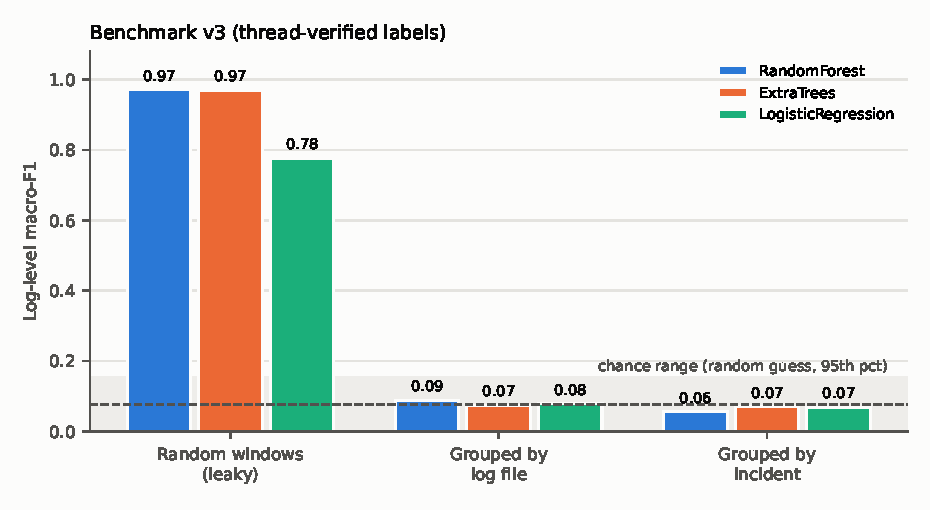
\includegraphics[width=0.85\linewidth]{figures/leakage_v3.pdf}
\caption{Same models, same data, three split protocols. The shaded band is
the frequency-random baseline up to its 95th percentile.}\label{fig:leak}
\end{figure}

\begin{table}[t]\centering\small
\caption{Benchmark v3 results (34 logs, 32 incidents). Model rows: mean
$\pm$ s.d. over 5 seeds. Rule rows: 95\% incident-cluster bootstrap CI.}
\label{tab:results}
\begin{tabular}{lccc}
\toprule
Method & Random windows & Grouped by log & Grouped by incident\\\midrule
RandomForest & $0.971\pm0.000$ & $0.088\pm0.006$ & $0.056\pm0.009$\\
ExtraTrees & $0.971\pm0.003$ & $0.074\pm0.002$ & $0.069\pm0.002$\\
Logistic regression & $0.777\pm0.053$ & $0.078\pm0.007$ & $0.069\pm0.001$\\\midrule
& \multicolumn{3}{c}{Macro-F1 (correct top-1 of 34)}\\\cmidrule{2-4}
Rule engine & \multicolumn{3}{c}{0.062 [0.014, 0.139] (4)}\\
Rules + fusion, CITA off & \multicolumn{3}{c}{0.054 [0.000, 0.124] (3)}\\
Rules + fusion, CITA on & \multicolumn{3}{c}{0.000 [0.000, 0.000] (0)}\\\midrule
Majority class & \multicolumn{3}{c}{0.038}\\
Frequency-random (mean / 95th pct) & \multicolumn{3}{c}{0.076 / 0.152}\\
\bottomrule
\end{tabular}
\end{table}

\textbf{Results} (Fig.~\ref{fig:leak}, Table~\ref{tab:results}):
\begin{itemize}
\item \textbf{H1 (leakage) is supported for every model.} Random window
      splits give 0.78--0.97; incident grouping gives 0.06--0.07.
\item \textbf{H2 (no skill) is supported.} No method exceeds the 95th
      percentile of the frequency-random baseline (0.152).
\item \textbf{H3 is supported.} CITA does not help: it changed 19 of 34 top-1
      rule diagnoses, and correct answers fell from 3 to 0.
\item \textbf{The explicit-label subset} (14 logs) gives the same picture:
      2/14 correct for rules, 0/14 with CITA.
\item \textbf{Earlier label versions} give the same staircase: 0.89 $\to$
      0.14--0.17 $\to$ 0.08--0.09 on v1, and 0.99--1.00 $\to$ 0.05 on v2.
\end{itemize}

\section{Error analysis}\label{sec:errors}
For the 10 verified \texttt{mechanical\_failure} logs, where a motor, ESC
or cable suddenly stopped producing thrust:
\begin{itemize}
\item \textbf{Rule engine:} predicts \texttt{power\_instability} 5 times and
      \texttt{motor\_imbalance} 2 times, and is correct once.
\item \textbf{With CITA:} predicts \texttt{motor\_imbalance} 6 times.
\end{itemize}
Both are \emph{consequences} of the failure. Current drops when a motor
stops, and the controller drives the remaining motors apart to compensate.
Onset-ordering cannot separate them from the cause, because they begin
within milliseconds of it. Better diagnosis therefore needs features that
model the failed actuator directly: a commanded output saturating at
maximum while its thrust contribution and current fall. Earliest-anomaly
heuristics are not enough.

\section{Limitations}
\begin{itemize}
\item The benchmark is small (34 logs), class-imbalanced and
      multicopter-heavy, and it inherits forum selection bias.
\item Labels come from a single automated annotator and have not been
      human-reviewed. Each is independently checkable, and a human
      spot-check is pending.
\item Many causes are tentative in their threads.
\item Fault onset times are not yet annotated.
\item A fully confirmatory test on incidents posted after registration is
      future work.
\end{itemize}

\section{Availability}
Code, registry, thread annotations with quotes, derived features, result
files and the pre-registration are public in the project repository.
\texttt{python training/paper\_eval.py} regenerates every table. Result
files record the exact commit and input hashes.

\bibliographystyle{plainnat}
\bibliography{references}
\end{document}
